% !TeX root = ../main.tex
% Add the above to each chapter to make compiling the PDF easier in some editors.
\chapter{Simulations}\label{chapter:simulations}

Simulation is the representation of the way a system or process functions. Simulations can be used for various purposes. We are using simulations for the following two main purposes:

\begin{enumerate}
 \item To check the validity of our implementations. For example, We have implemented the Access Point capability. An Access Point can have three modes and there are certain rules of connectivity. We are using simulations to verify that these rules of connectivity are correctly implemented.
 \item Inference of results from the output of simulations. For example, building on the example of Access Points, we are using simulations to explore the impact of access points on the performance of geo-based information sharing.
\end{enumerate}

To make things easier, we have divided the simulations into a number of scenarios. Each scenario is used for either validation of the implementation or inference of results as mentioned above. One thing to keep in mind is that since we have to run a lot of simulations, all the simulations are run in batch (non-GUI) mode and the result is written to different reports. All the reports are stored on disk as text files.

\section{Concepts}
The following concepts are necessary to understand how the simulations work as well as the generated report files.

\begin{itemize}
\item \textbf{Warmup time}: A real-world system normally takes some time (after it is started) to come to a stable state. In order to simulate this, we are making use of the warmup time. Any events generated during this time (such as Message Generation, Replication etc.) are ignored by the reports.
\item \textbf{Cooldown time}: Cooldown time refers to the time period we are allowing the system to cool down. In other words, cooldown time ensure that message created before the start of the cooldown time have enough time to live (TTL) before the simulation ends. The cooldown time equal to TTL (time to live) of the messages. All the events generated during this time (such as Message Generation, Replication etc.) except \textit{MessageDeleted} are ignored by the reports. \textit{MessageDeletion} event will not be ignored for those message created before the cooldown time starts. We have achieved the following using cooldown time:
\begin{enumerate}
	\item Any messages created after the cooldown time starts are not recorded in the report. This gives consistency to the report and makes it more reliable. For example, any message created after the cooldown time starts (1500 minutes timestamp) might still be in the system when the simulation time completes (because their TTL is 300 minutes).
	\item It allows the messages created before cooldown time to be safely deleted or dropped. An edge case example would be messages created right before the cooldown starts (at 1500 minutes timestamp). In case these messages are not dropped before the end of the simulation, they would be dropped right before the end of simulation due to the expiry of their time to live (TTL).
\end{enumerate}

Let's explain this with the help of an example:
Consider we are running a simulation for 1800 minutes and the TTL (time to live) for messages is 300 minutes. The cooldown time is equal to the TTL (time to live) of messages which would mean that the cooldown will start right after the 1500th-minute mark.
\end{itemize}

\section{Scenarios}
As mentioned above, We have grouped the simulations in Scenarios. Each of the Scenario is responsible for different components of the simulation. Below is a brief introduction of the scenarios:

\begin{enumerate}
	\item \textbf{Scenario 1.x}: Broadly speaking, these scenarios are used for validation of our access points logic and exploring the impact of access points on the performance of geo-based information sharing.
	\item \textbf{Scenario 2}: These scenarios are used to evaluate how snapping to access point affects the availability of a floating message in a Delay Tolerant Network (DTN).
\end{enumerate}
\subsection{Scenario 1.1: Validation of Access Point based connections}
As mentioned in the earlier chapters, one of our goals was to implement Access Points based connectivity in the ONE Simulator. The main idea is to simulate the Access Point that we use in normal networks. It has already been mentioned that an Access Point can have three modes of operations: Access Point (AP), Ad-hoc and Station Adapter (SA). Below are the conditions/rules that are used for connectivity:
\begin{enumerate}
	\item Station Adapters (SA) can only connect to Access Points (APs). The main idea is that Access Points serve different Station Adapters. A related example would be a mobile device connected to a wifi router. In this example, the mobile device is the Station Adapter (SA) and the wifi router is the Access Point (AP).
   	\item A device in Ad-hoc mode can only connect to another device in Ad-hoc mode.
\end{enumerate}
In order to make sure that the above conditions/rules hold, We have created a simulation that records the connectivity (Connection UP and DOWN) when the connectivity status between the two nodes change. We are using a special report for this purpose which is basically recording the connectivity events for only Access-Point enabled clients. It is worth mentioning here that the normal clients (non-Access Point enabled) can co-exist with Access Point enabled clients but this report will not record connectivity events of the normal clients. We call this the \textit{ConnectivityWifiONEReport}.
\vspace{3mm}
\begin{lstlisting}[language=java]
public class ConnectivityWifiONEReport extends ConnectivityONEReport {
	public static final String HEADER = "simTime, host1, mode, host2, mode, up/down";
	public ConnectivityWifiONEReport() {
		init();
	}
	@Override
	public void init() {
		super.init();
		write(HEADER);
	}
	@Override
	public void hostsConnected(DTNHost h1, DTNHost h2) {
		if(h1 instanceof DTNHostWithWifi || h2 instanceof DTNHostWithWifi) {
			write(createTimeStamp() + "," + h1.toString() + "," + ((DTNHostWithWifi)h1).getModeName() + "," + h2.toString() + "," + ((DTNHostWithWifi)h2).getModeName() + "," + "UP");
		}
	}
	@Override
	public void hostsDisconnected(DTNHost h1, DTNHost h2) {
		if(h1 instanceof DTNHostWithWifi || h2 instanceof DTNHostWithWifi) {
			write(createTimeStamp() + "," + h1.toString() + "," + ((DTNHostWithWifi)h1).getModeName() + "," + h2.toString() + "," + ((DTNHostWithWifi)h2).getModeName() + "," + "DOWN");
		}
	}
}
\end{lstlisting}
\captionof{lstlisting}{Code for ConnectivityWifiONEReport}
\vspace{5mm}
The above listing shows the implementation for \textit{ConnectivityWifiONEReport}. Below is a summarized explanation of the above code:
\begin{itemize}
	\item The \textit{ConnectivityWifiONEReport} inherits from the \textit{ConnectivityONEReport} (which is responsible for recording the connectivity reports of all the nodes).
	\item The HEADER is basically the first line written to the report file. It provides context to any user reading the report so that anyone reading the report understand what each value correspond to.
	\item \underline{hostsConnected} function writes the connection UP status to the report file only if at least one of the hosts is an Access Point enabled host (also called \textit{DTNHostwithWifi}).
	\item \underline{hostsDisconnected} function writes the connection DOWN status to the report file only if at least one of the hosts is an Access Point enabled host (also called \textit{DTNHostwithWifi}).
\end{itemize}

\subsection{Scenario 1.2: Modeling Munich City with Access Points}
The main purpose of this scenario is to model the Munich city (central part of the city) with as well as without Access Points. The main purpose is to simulate both of these sub-scenarios with similar parameters and then compare the results to study the impact of access points on the performance of geo-based information sharing. Below is an explanation of these sub-scenarios:
\begin{enumerate}
	\item \textbf{Access Points}: In this sub-scenario, Publicly available access points are modeled on the map of Munich city. In order to make the simulations fast enough, we are utilizing just a subset of those Access Points.
	\item \textbf{No Access Points}: In this sub-scenario, we are not using any access points. In order to have the same configuration for both the scenarios, we are modeling the access points as stationary nodes/hosts on the map.
\end{enumerate}
\vspace{1mm}
In order to get comparable results, both of these sub-scenarios are simulated using a set of different parameters. The following list explains each of these parameters in details:

\begin{enumerate}
	\item \textbf{Message Size}: Message Size plays a vital role in the simulations. Since each node can have a limited amount of space, message size indirectly depicts the capacity of these nodes. The smaller the message size, the more messages a node can store without dropping any message, thus a higher storage capacity. We are using the message sizes \textit{1 Kilobyte (1k)}, \textit{50 Kilobyte (50k)} and \textit{1 Megabyte (1M)} for our simulations. We are using \textit{1 Kilobyte(1k)} to give our hosts virtually unlimited storage space and we are using \textit{1 Megabyte (1M)} to give very limited storage space to our hosts.
	\item \textbf{Message Availability and Replication Zone}: Message Availability Zone defines the area where a message can exist. Message Replication Zone defines the area where a message can be replicated (copied to) other nodes. It has a direct impact on the life of the message (as any message that leaves this zone is dropped). We are using a radius of \textit{100}, \textit{200} and \textit{300} for message availability and replication zones. We are using \textit{300} to simulate message availability over a bigger area and \textit{100} to simulate message availability over a relatively smaller area.
	\item \textbf{The number of Hosts/Nodes}: The number of hosts/nodes also play a vital role in the simulations. We are using different sets of configuration for this purpose. Below is an explanation:
		\begin{itemize}
			\item \underline{Cars}: Since our simulation area mostly consists of the pedestrian zone, we are not simulating a lot of cars. We are using either 30 or 50 hosts as cars.
			\item \underline{Pedestrians}: In case the number of cars is less than 50, the number of pedestrians is 1.5 times the number of cars. Otherwise, the number of pedestrians is 100. Pedestrians are the main component of our simulations as we are using a map with a high percentage of pedestrian zone.
			\item \underline{Access Points/Stationary Nodes}: In case the number of cars is less than 50, we are using 64 access points/stationary nodes. Otherwise, we are using 132 access points/stationary nodes.
      \item The main objective is run the simulations with a lower as well as a higher density of hosts. This enable us to study network performance (measured in fraction of TTL) in both of these conditions. We have chosen the above numbers to fulfill this objective.
		\end{itemize}
\end{enumerate}

For both of these sub-scenarios, we are utilizing the \textit{FloatingMessageSummaryReport}. The main purpose of this report is to record the creation, deletion time, time to live, life (the time between the creation of the message to the deletion of the last copy), total copies as well as the number of dropped copies of the message. The messages are dropped in case there is no more space left. One thing to note here is that creation time is the time when the message is first created while deletion time is the time when the last copy of the message is deleted.

\begin{lstlisting}[language=java]
	protected boolean isCooldown(Message m) {
		double cooldownTime = m.getInitTtlInSeconds();
		return (SimScenario.getInstance().getEndTime() - getSimTime()) <= cooldownTime ;
	}

	public static final String HEADER = "msgId, created_on, deleted_on, ttl, life, totalCopies, dropped";

	public void newMessage(Message m) {
		if(isWarmup() || isCooldown(m))
			return;

		MessageSummary messageSummary = new MessageSummary(m.getInitTtlInSeconds());
	    messagesSummary.put(m.getId(), messageSummary);
	}

	public void messageTransferred(Message m, DTNHost from, DTNHost to, boolean firstDelivery) {
		if(isWarmup() || isCooldown(m))
			return;

		MessageSummary messageSummary = messagesSummary.get(m.getId());
		//This makes sure that we only count messages which were created before cooldown
		if(messageSummary != null) {
			messageSummary.incrementCount();
			messagesSummary.put(m.getId(), messageSummary);
		}
	}

	public void messageDeleted(Message m, DTNHost where, boolean dropped) {
		if(isWarmup())
			return;

		MessageSummary messageSummary = messagesSummary.get(m.getId());
		//This makes sure that we only count messages which were created before cooldown
		if(messageSummary != null) {
			messageSummary.decrementCount(dropped);
			messagesSummary.put(m.getId(), messageSummary);
		}
	}
\end{lstlisting}
\captionof{lstlisting}{Code snippets from FloatingMessageSummaryReport and Report}
\vspace{5mm}
The above listing shows code snippet from \textit{FloatingMessageSummaryReport} and \textit{Report}. Below is a summarized explanation of the above code:
\begin{itemize}
	\item \underline{isCooldown} function returns true if the cooldown period has started otherwise it returns false.
	\item \underline{newMessage} function reports when a new message is created. The message creation event is not recorded in case it is the warm-up time or the cool down time.
	\item \underline{messageTransferred} function reports when the message is replicated to another host. In the case of replication, a copy of the message is created and sent to the new host. The transfer event is not recorded in case it is the warm-up time or the cool down time.
	\item \underline{messageDeleted} function reports when a copy of the message is deleted/dropped by a host. The transfer event is not recorded in case it is the warm-up time or the cool down time. \newline \textit{MessageSummary messageSummary = messagesSummary.get(m.getId());} will only return a non-null value if the message was created before the cooldown time otherwise it will return \textit{null}. The deletion event is only recorded if this line returns a non-null response.
\end{itemize}

\subsection{Scenario 2: Simulating Snapping to Access Points}
The main purpose of this scenario is to simulate the snapping to access point and determine how does it affect the availability of the messages in a Delay Tolerant Network (DTN). We are also using the Publicly available access points data for this scenario.

We are using the same combination of parameters as \textit{Scenario1}. \newline
We are using two different types of reports for this scenario. The first report is \textit{FloatingMessageSnapToAPSummaryReport} while the second is \textit{FloatingMessageAnchorPointsReport}. The following listing explains both fo these reports:

\begin{itemize}
	\item \underline{FloatingMessageSnapToAPSummaryReport}: This report records snapping of the message to the access point. It records the creation and deletion time, time to live (TTL), life (the time between the creation of the message to the deletion of the last copy), count of dropped copies and number of message copies snapped to 0,1,2 or 3 access points.
	\item \underline{FloatingMessageAnchorPointsReport}: This report also records snapping of the message to the access point but with a different perspective. Instead of recording the number of access points the message is snapped it, it records the original anchor as well as all the snapped anchors for a message.
\end{itemize}

\vspace{2mm}
The following listing shows the relevant code snippet from \textit{FloatingMessageSnapToAPSummaryReport}.


\begin{lstlisting}[language=java]
	public void messageDeleted(Message m, DTNHost where, boolean dropped) {
		if(isWarmup())
			return;

		MessageSummary messageSummary = messagesSummary.get(m.getId());
		if(messageSummary != null) {
			messageSummary.decrementCount(m);
			messageSummary.updateSnapCount(m, dropped);
			if(dropped)
				messageSummary.droppedMessagesCount++;
			messagesSummary.put(m.getId(), messageSummary);
		}
	}

	public void messageTransferredWithNewAnchor(Message m, Message replicatedWithNewAnchor, DTNHost from, DTNHost to) {
		if(isWarmup() || isCooldown(m))
			return;

		MessageSummary messageSummary = messagesSummary.get(m.getId());
		if(messageSummary != null)
			messagesSummary.put(m.getId(), messageSummary);
	}

	@Override
	public void done() {
	    double sum = 0;
	    double count = 0;
	    for(String key: messagesSummary.keySet()) {
	    	count ++;
	    	MessageSummary messageSummary = messagesSummary.get(key);
	    	write(key+","+messageSummary.toString());
	    	sum += (messageSummary.deletionTime - messageSummary.creationTime) / 60.0;
	    }

	    write("Average,,,," + sum / count);
	    super.done();
	}
\end{lstlisting}
\captionof{lstlisting}{Code snippets from FloatingMessageSnapToAPSummaryReport}
\vspace{5mm}
The above listing shows code snippet from \textit{FloatingMessageSnapToAPSummaryReport}. Below is a summarized explanation of the above code:
\begin{itemize}
	\item \underline{messageDeleted} function has two main tasks. It records deletion of the message and it also records the number of access points the message is snaped to for those messages created before the cooldown time.  We are recording the number of access points the message is snapped to here because this is the only place after which this information does not change for that copy of the message (as the copy has been deleted).
	\item \underline{messageTransferredWithNewAnchor} function reports when a copy of the message is snapped to a new access point. The transfer event is not recorded in case it is the warm-up time or the cool down time.
	\item \underline{done} This method summarizes all the information and writes it to the report file. It also writes the average life of message (for this simulation) to the file.
\end{itemize}

The code for \textit{FloatingMessageAnchorPointsReport} is roughly the same, however, the only difference is that \textit{messageTransferredWithNewAnchor} records the anchor point (location) of the \textit{access point} the message is snapped to.


\section{Results}
Before going into the discussion of results, below is a list of the different parameters we are using for our simulations:
\begin{enumerate}
  \item \textbf{Message Size}: We are message size of \textit{1 Kilobyte (1k)}, \textit{50 Kilobyte (50k)} and \textit{1 Megabyte (1M)}.
  \item \textbf{Message Availability and Replication Zone}: We are using \textit{100}, \textit{200} and \textit{300} meters for both availability and replication zones.
  \item \textbf{The number of Hosts/Nodes}: We are using either \textit{Low}(126 hosts) or \textit{High} (282 hosts) for the nodes count configuration.
  \item \textbf{Simulation Runs}: We run the simulations for 100-120 times for each of the parameter combination.
\end{enumerate}

We are using all the 18 combinations of the above three parameters (from 1k-100-L to 1M-300-H). These combinations will be listed in the \textit{Message Size-Availability and Replication Zone-Nodes Count-Number of Hosts}) format.\newline\newline
In each of the following scenarios, the performance of the network (measured in a fraction of Time-To-Live (TTL))is our benchmark for comparison. We will start with benchmarking each parameter individually, then a combination of two parameters and finally all of the parameters together (if needed).
\subsection{Scenario 1}
In this Scenario, we are mainly interested in understanding and evaluating the effect of access points based setup on delay tolerant networks. To achieve this goal, we have run a number of simulations (with different parameters as stated above) which we will analyze below.
\subsubsection{Message Size vs The fraction of TTL (time to live)}
Message size represents two important features of the system. The first is the message size itself and the second is capacity of the nodes. However, both of these are inverse relationships (the smaller the message size, the higher the capacity of the node and vice versa). \emph{Figure}~\ref{fig:scenario1_message_size} plots the message life vs the fraction of TTL (Time To Live), regardless of the other two parameters i.e. the availability zone and the number of hosts. This figure shows that traditional hosts perform better than the access points enabled hosts when the message is smaller in size (or the nodes have higher capacity). As the message size increases (or the node capacity decreases), the performance of traditional hosts decrease while that of access points enabled hosts remains almost the same until message size of 50k. After the 50k mark, enabled access points starts to perform better than their traditional counterparts. So the access points enabled hosts perform much better when the message size is higher than 50k (or when nodes have lower capacity). In short, the performance of the wifi enabled hosts increase with increase in message size (or decrease in node capacity).

\begin{figure}[h]
  \centering
  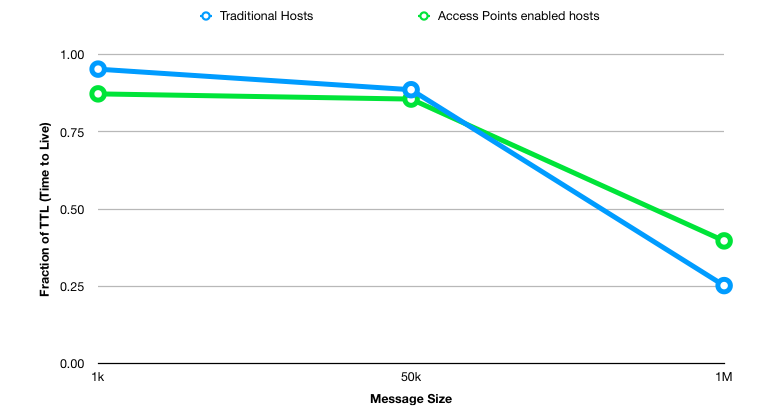
\includegraphics[scale=0.45]{./figures/scenario1_message_size}
  \caption{Message Size vs The fraction of TTL (time to live) with 90-95\% accuracy}
  \label{fig:scenario1_message_size}
\end{figure}
\subsubsection{Message Availability/Replication Zone vs The fraction of TTL (time to live)}
Availability/Replication zones represent the area where a message can exist (and copied to other hosts). {\emph{Figure}~\ref{fig:scenario1_availability_zone} plots the availability zone vs the fraction of TTL (time to Live), regardless of the other two parameters i.e. message size and the number of hosts. This figure shows that traditional hosts perform better than the access points enabled hosts when the availability/replication zone size is smaller. As the availability/replication zone size increases, the performance of access point enabled hosts increases at a good rate while that of the traditional hosts almost stay the same until 200 meters and then increases by a relatively small rate (w.r.t wifi enabled access points). In short, the performance of wifi enabled hosts increase with increase in the availability zone size.
\begin{figure}[H]
  \centering
  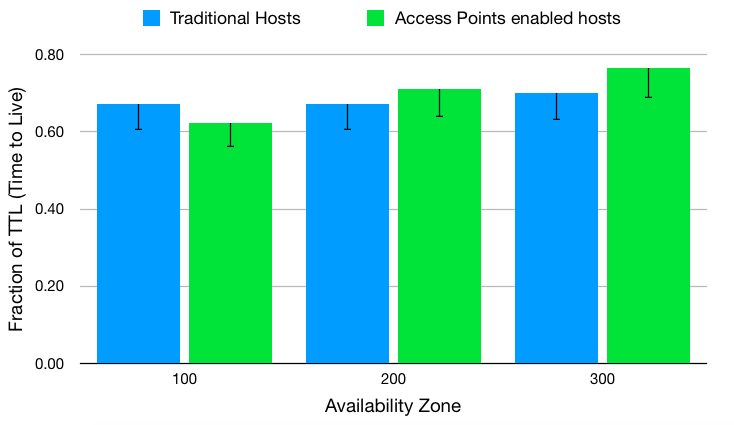
\includegraphics[scale=0.45]{./figures/scenario1_availability_zone}
  \caption{Availability Zone vs The fraction of TTL (time to live)}
  \label{fig:scenario1_availability_zone}
\end{figure}
\subsubsection{The number of hosts vs The fraction of TTL (time to live)}
The number of hosts used is the simulations basically refer to the density of the hosts (which is either \textit{Low} or \textit{High}). \emph{Figure}~\ref{fig:scenario1_availability_zone} plots the availability zone vs fraction of TTL (time to live), regardless of the other two parameters i.e. message size and the number of hosts.
\begin{figure}[H]
  \centering
  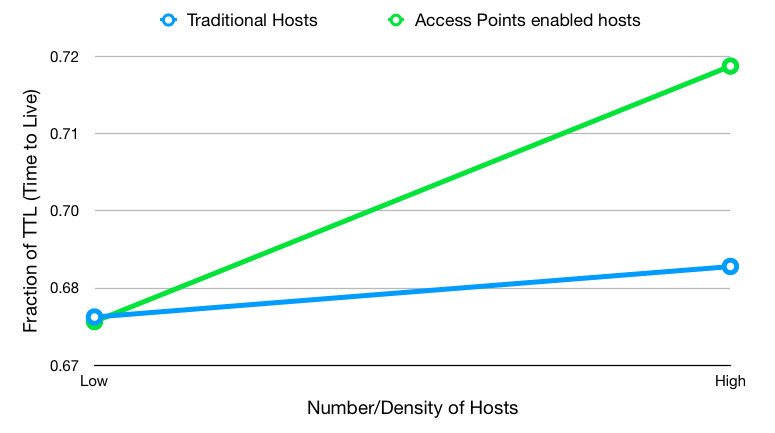
\includegraphics[scale=0.45]{./figures/scenario1_hosts_count}
  \caption{Number of hosts vs The fraction of TTL (time to live)}
  \label{fig:scenario1_number_of_hosts}
\end{figure}
The above figure shows that traditional hosts perform better than the access points enabled hosts when the availability/replication zone size is smaller. As the availability/replication zone size increases, the performance of access point enabled hosts increases at a good rate while that of the traditional hosts increase by a relatively small rate (w.r.t wifi enabled access points). In short, the performance of wifi enabled hosts increase with increase in size of the availability zone size. Increasing the number of hosts indicate an increase in resources that can hold and replicate the message, causing in an increase in the average message life. The performance is much better in access points enabled hosts because the hosts working as access points do not generate any new messages and are just responsible for storing and routing of the message.
\subsubsection{Message size and Availability zone size vs The fraction of TTL (time to live)}
\emph{Figure}~\ref{fig:scenario1_message_size} and ~\ref{fig:scenario1_availability_zone} shows that message size and availability zones both have an effect on the performance (measured in a fraction of TTL (time to live)) of the network. In order to figure out which parameter has more influence on the system, we plot them together and then try to figure out which parameter has the main influence on the network performance.
\begin{figure}[H]
  \centering
  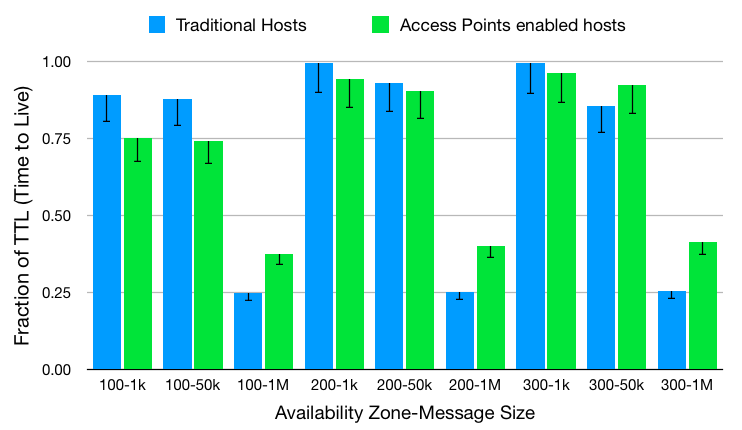
\includegraphics[scale=0.55]{./figures/scenario1_message_size_availability_zone_1}
  \captionof{figure}{Availability Zone-Message Size vs The fraction of TTL (time to live)}
  \label{fig:scenario1_message_size_availability_zone_1}
\end{figure}
\emph{Figure}~\ref{fig:scenario1_message_size_availability_zone_1} plots the message size and availability zone vs fraction of TTL (time to live), regardless of the number of hosts. These charts/figures show that message size has the dominant effect on the network performance (measured in a fraction of TTL (time to live)). To come to this conclusion, we divide the graph into three main components w.r.t the availability zones. By looking into each of the components, there is a significant change in the message availability as the message size changes. Thus, confirming our observation that message size is the main component while the availability zone is a supplementary component. In other words, the performance (fraction of TTL (time to live) depends mainly on message size.\newline
Our conclusion is supported by \emph{Figure}~\ref{fig:scenario1_message_size_availability_zone_2}, where we interchange the two parameters, to have the chart visually grouped by message size instead of the availability zone.
\begin{figure}[H]
  \centering
  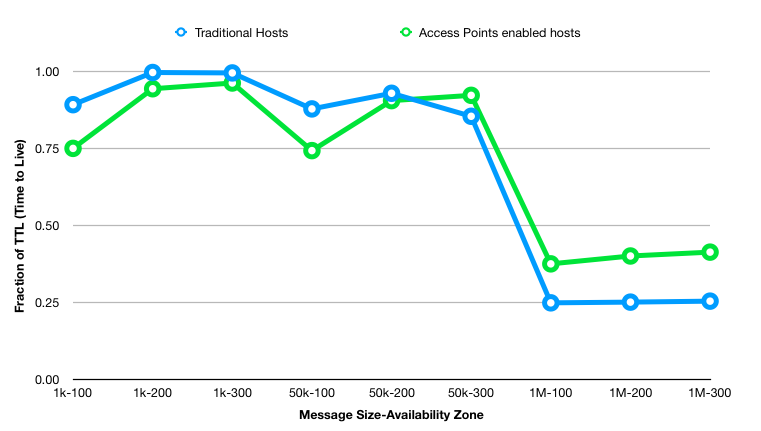
\includegraphics[scale=0.55]{./figures/scenario1_message_size_availability_zone_2}
  \captionof{figure}{Message Size-Availability Zone vs The fraction of TTL (time to live)}
  \label{fig:scenario1_message_size_availability_zone_2}
\end{figure}
\subsection{Scenario 2}
In this scenario, our main goal is to compare the network performance (measured in a fraction of TTL (time to live)) with respect to the number of access points a message can snap to (also known as \textbf{k}).
\subsubsection{Message Size, Availability Zone, Hosts Count vs The fraction of TTL (time to live)}
Let us start by plotting the fraction of TTL (time to live) against all the three parameters (message size, availability zone, and  hosts count). \emph{Figure}~\ref{fig:scenario2_1_all_parameters} plots all the variables against the fraction of TTL (time to live). This figure shows \textit{snapping to access points} perform better than \textit{no snapping}. Examining the figure closely reveals that the difference in performance is negligible in some cases while it is quite substantial in other cases.
\emph{Figure}~\ref{fig:scenario2_1_all_parameters} reveals that snapping to access points perform better than no snapping. We now need to understand if increasing the number of access points a message can snap to (also known as \textbf{k}) really increases the fraction of TTL (time to live).
\begin{figure}[H]
  \centering
  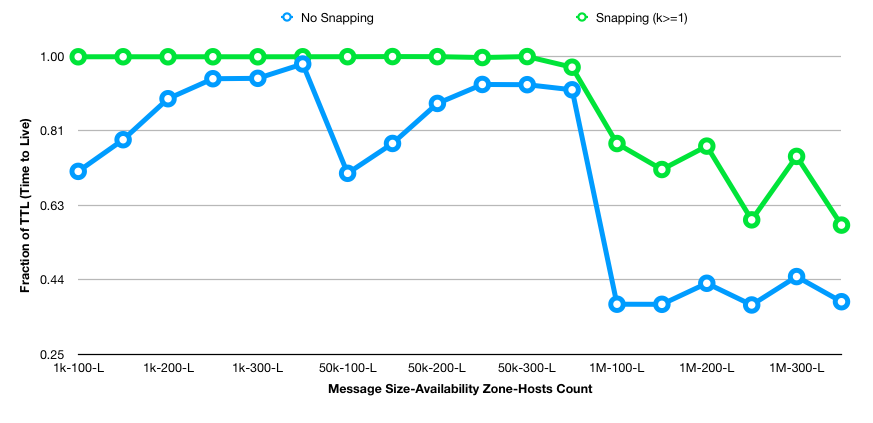
\includegraphics[scale=0.41]{./figures/scenario2_1_all_parameters}
  \captionof{figure}{Message Size-Availability Zone-Hosts Count vs The fraction of TTL (time to live)}
  \label{fig:scenario2_1_all_parameters}
\end{figure}
\emph{Figure}~\ref{fig:scenario2_1_2_all_parameters} plots the fraction of TTL (time to live) w.r.t the number of access points the message is snapped to (\textbf{k}). We are plotting for all the k-values we are supporting i.e. 0,1,2,3. In case of smaller message size (or higher node capacity), increasing \textbf{k} does not have any effect on the fraction of TTL (time to live). However, in case of large message size (>= 1M), increasing \textbf{k} have a positive effect on the fraction of TTL (time to live).
\begin{figure}[H]
  \centering
  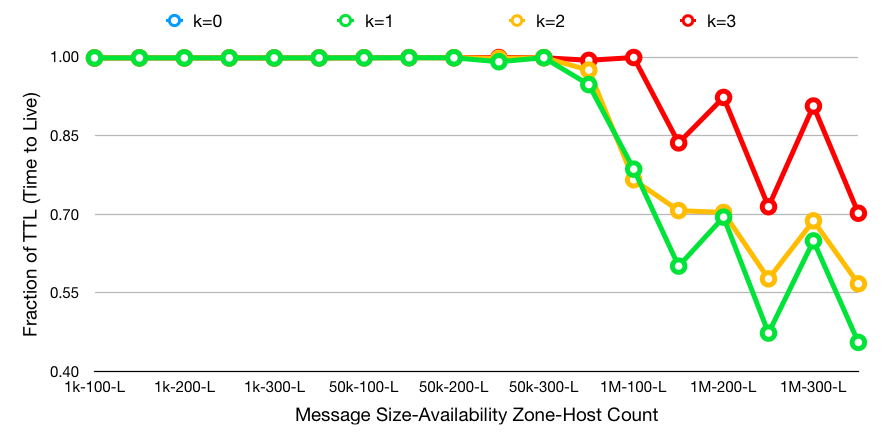
\includegraphics[scale=0.4]{./figures/scenario2_1_2_all_parameters}
  \captionof{figure}{k (number of access points a message can snap to) vs The fraction of TTL (time to live)}
  \label{fig:scenario2_1_2_all_parameters}
\end{figure}
In order to ascertain if the behavior depicted in \emph{Figure}~\ref{fig:scenario2_1_all_parameters} and \emph{Figure}~\ref{fig:scenario2_1_2_all_parameters}, we will take each of the individual components and evaluate its effect on the fraction of TTL (time to live) for k = 0,1,2,3.
\newpage
\subsubsection{Message Size vs The fraction of TTL (time to live)}
\emph{Figure}~\ref{fig:scenario2_2_message_size} plots message size against the fraction of TTL (time to live). This figure shows that the case of no snapping (\textit{k=0}) performs worse than the other cases (\textit{k>0}). It also shows that when the message size is smaller (up to 50k), increasing \textbf{k} does not have any effect on the fraction of TTL (time to live). However, as the message size increases, increasing \textbf{k} have a positive effect on the fraction of TTL (time to live).

\begin{figure}[H]
  \centering
  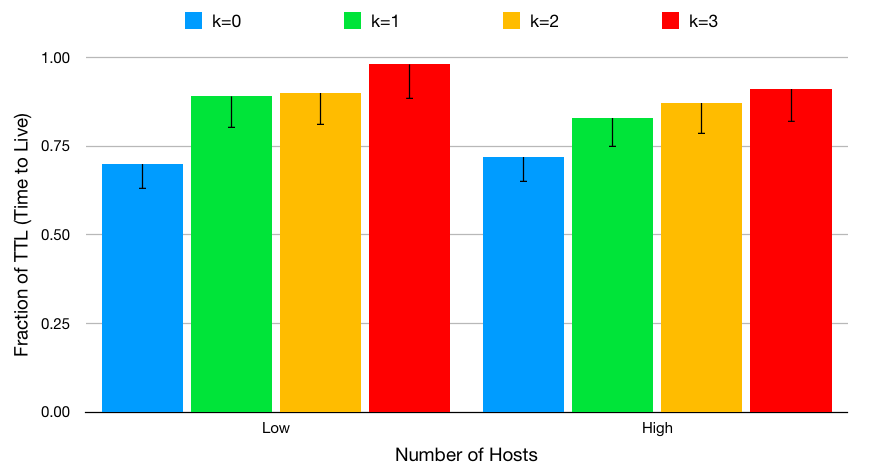
\includegraphics[scale=0.4]{./figures/scenario2_2_message_size}
  \captionof{figure}{Message Size vs The fraction of TTL (time to live)}
  \label{fig:scenario2_2_message_size}
\end{figure}

\subsubsection{Availability Zone vs The fraction of TTL (time to live)}
\emph{Figure}~\ref{fig:scenario2_3_availability_zone} plots availability size against the fraction of TTL (time to live).
\begin{figure}[H]
  \centering
  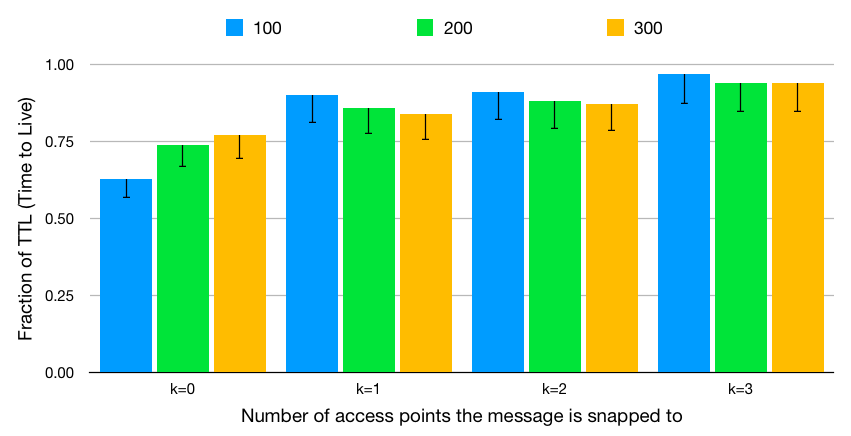
\includegraphics[scale=0.39]{./figures/scenario2_3_availability_zone}
  \captionof{figure}{Availability Zone vs The fraction of TTL (time to live)}
  \label{fig:scenario2_3_availability_zone}
\end{figure}
The above figure shows that the case of no snapping (\textit{k=0}) always performs worse than the other cases (\textit{k>0}). It also shows that increasing \textbf{k} (when changing the availability zone) always have a positive effect on the fraction of TTL (time to live). However, one thing to note is that increasing the availability zone does not cause a minor decrease in network performance for access points enabled hosts. The main reason might be: as the availability zone increases, the access points would have to deal with more messages, resulting in more messages being dropped.
\subsubsection{Number of Hosts vs The fraction of TTL (time to live)}
\emph{Figure}~\ref{fig:scenario2_4_hosts_count} plots number of hosts against the fraction of TTL (time to live). This figure shows that the case of no snapping (\textit{k=0}) always performs worse than the other cases (\textit{k>0}). It also shows that the increasing \textbf{k} (when changing the number of hosts) always have a positive effect on the fraction of TTL (time to live). In other words, higher values of \textbf{k} almost always correspond to a better fraction of TTL (time to live) than lower values.
\begin{figure}[H]
  \centering
  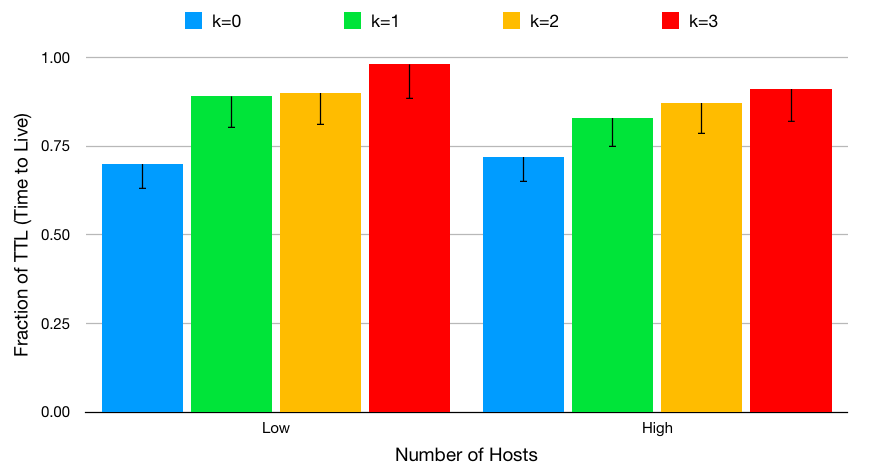
\includegraphics[scale=0.39]{./figures/scenario2_4_hosts_count}
  \captionof{figure}{Number of Hosts vs The fraction of TTL (time to live)}
  \label{fig:scenario2_4_hosts_count}
\end{figure}
\vspace{1mm}
This marks the completion of our simulations and the analysis of their results. Using the analysis in this chapter, We would infer the results and discuss them in the next chapter.
